% Added link to preamble
\documentclass[12pt]{article}
\usepackage[utf8]{inputenc}
\usepackage{blindtext}
\usepackage{graphicx}
\usepackage{tabularx}
\usepackage{authblk}
%\usepackage{natbib}
\usepackage{xcolor}
\usepackage{float}
\usepackage{amsmath}
\usepackage[english]{babel}
\usepackage{graphicx} % Required for inserting images
\usepackage[paperheight=16cm,paperwidth=12cm,textwidth=8cm]{geometry}
\usepackage[flushleft]{threeparttable,booktabs}

\usepackage[
        backend=biber,
        style=authoryear-comp,
        sorting=nyt,
        style=apa
    ]{biblatex}
 \addbibresource{references.bib}


 \geometry{
 a4paper,
 total={170mm,257mm},
 left=30mm,
 right=30mm,
 top=30mm,
 bottom=30mm
 }

% Keywords command
\providecommand{\keywords}[1]
{
  \small	
  \textbf{\textit{Keywords---}} #1
}

\graphicspath{{plot/}}



\addbibresource{}
\documentclass{article}


\title{Names diffusion and social class}
\author{}
\date{May 2023}

\begin{document}

\maketitle

\section{Introduction}


\begin{figure}[H]
    \centering
    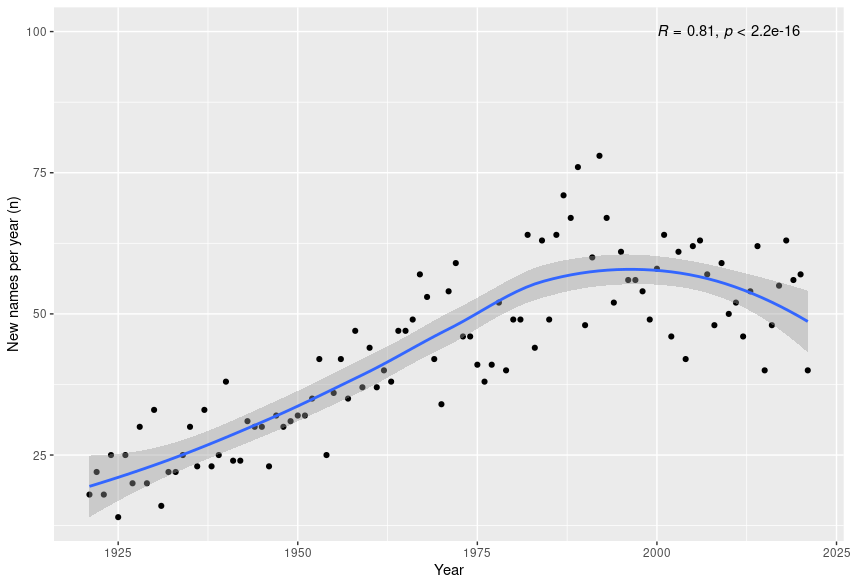
\includegraphics[width=13cm]{plot/new_names_year.png}
    \caption{Number of new names per year in Chile (1920-2022)}
    \label{}
\end{figure}


\begin{figure}[H]
    \centering
    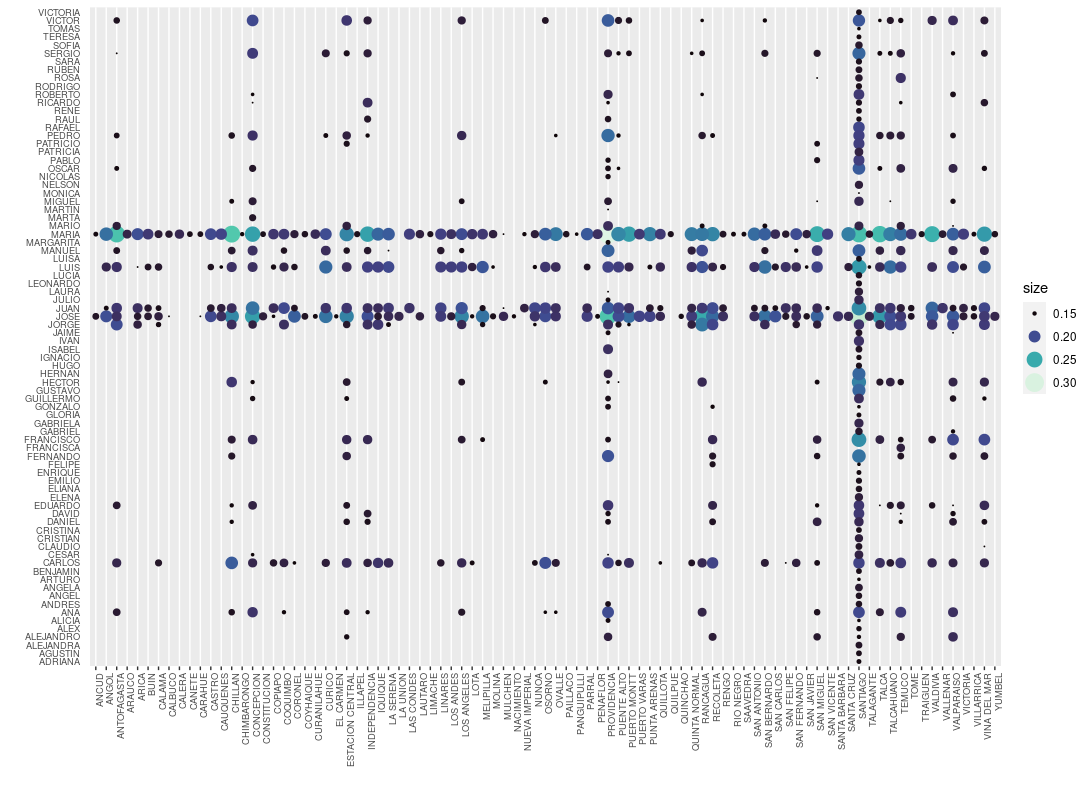
\includegraphics[width=13cm]{plot/name_commune.png}
    \caption{top names per commune in Chile (1920-2022)}
    \label{}
\end{figure}


\section{Methodology}

Podemos representar ejemplos de cómo los trabajadores cambian de trabajo como redes complejas. En esta red, cada tarea está representada por un nodo y cada ruta entre dos nodos representa la cantidad de trabajadores que se movieron de una tarea a otra. Los pesos de los bordes pueden no ser iguales, lo que significa que la cantidad de trabajadores que se mueven de un trabajo a otro puede no ser igual a la cantidad de trabajadores que se mueven en la dirección opuesta.

La matriz adyacente a esta red es una función normal de la tabla de enrutamiento. Esto se debe a que cada entrada en la matriz de adyacencia, \(w_ij \)  , representa la cantidad de trabajadores que pasaron del trabajo \( i\) al trabajo \( j \). Entonces, pensar en una tabla de enrutamiento como una red ponderada es solo otra forma de presentar la misma información.

Aquí hay un ejemplo de cómo podría funcionar esto. Digamos que tenemos un grupo de empleados y queremos hacer un seguimiento de cómo cambian sus trabajos con el tiempo. Podemos comenzar creando una red con un nodo para cada evento. Entonces podemos dar a cada lado de la red un peso que represente el número de trabajadores que se trasladaron de un trabajo a otro. Por ejemplo, si 100 trabajadores pasan del trabajo A al B, asignaríamos el peso a los 100 nodos que conectan los nodos A y B.

Podemos determinar cómo cambia la red con el tiempo actualizando los valores de umbral. Por ejemplo, si 50 trabajadores pasan del trabajo B al C, actualizaremos los pesos de borde que conectan los nodos B y C a 50.

Al observar los cambios en la red a lo largo del tiempo, podemos comprender mejor cómo los trabajadores se mueven entre trabajos. Esta información se puede utilizar para informar políticas para mejorar los resultados del mercado laboral. La idea de ver una tabla de flujo como una red tiene varios puntos importantes. Primero, nos permite considerar el flujo de información, influencia y otros recursos a través de la red. Esto se debe a que Internet no es solo una estructura fija; Estos son los sistemas dinámicos a través de los cuales fluyen los recursos.

En segundo lugar, pensar en la tabla de enrutamiento como una red nos permite ir más allá de las conexiones directas y considerar múltiples formas de conexión entre nodos. La razón es que el flujo de recursos a través de la red puede ser indirecto, ya que los recursos pueden fluir de un nodo a otro a través de un nodo intermedio. Tercero, pensar en la tabla de flujo como una red nos permite incluir información sobre la estructura de toda la red en nuestro análisis. Esto se debe a que la interfaz de red puede afectar el flujo de recursos a través de la red.

Aquí hay algunos ejemplos de cómo usar el concepto de una tabla de viaje como una red para responder preguntas de investigación:

Podemos utilizar el concepto de difusión para estudiar cómo se difunde la información sobre nuevos puestos de trabajo en la red. Por ejemplo, podemos ver cómo un nuevo proceso de referencia se extiende a las redes de amigos y colegas[1].

Podemos usar el concepto de flujo para estudiar cómo se mueve la influencia a través de una red. Por ejemplo, podemos determinar qué tan rápido se propaga el apoyo a una nueva política a través de una red de activistas políticos[2].

Podemos usar el concepto de flujo para estudiar cómo se propagan nuevas ideas o nuevas ideas a través de redes. Por ejemplo, podemos determinar qué tan rápido se propaga el uso de las nuevas tecnologías en las redes empresariales[3].

Al ver un diagrama de flujo como una red, podemos obtener una comprensión más profunda de cómo la información, la influencia y otros recursos se mueven en la sociedad. Esta comprensión se puede utilizar para desarrollar estrategias para mejorar los flujos de recursos y promover el desarrollo social y económico[1] [2] [3]. 


\begin{table}[H]
\centering
\begin{tabularx}{\textwidth}{p{5cm}|p{9cm}}
\hline
\textbf{Concepto} & \textbf{Descripción} \\
\hline
Red ponderada & Representación de los patrones de cambio de ocupación de los trabajadores mediante una red donde cada ocupación es un nodo, y los bordes representan los trabajadores que se trasladan entre ocupaciones, con pesos asimétricos. \\
\hline
Matriz de adyacencia & Tabla que muestra el número de trabajadores que se mueven de una ocupación a otra, representa la red ponderada de movilidad ocupacional. \\
\hline
Conceptualización de la tabla de movilidad como una red & La tabla de movilidad puede ser conceptualizada como una red ponderada, lo que permite un enfoque diferente para representar y analizar la movilidad ocupacional. \\
\hline
Flujo de información e influencia en la red & La representación de la movilidad ocupacional como una red ponderada permite analizar el flujo de información y recursos a través de la red, considerando las conexiones directas e indirectas y la estructura general de la red. \\
\hline
Implicaciones de la conceptualización de la tabla de movilidad como una red & La representación de la movilidad ocupacional como una red ponderada permite el análisis del flujo de recursos, como información, influencia y otros recursos, y su propagación a través de la sociedad. Esto puede tener implicaciones importantes para el diseño de políticas y el desarrollo social y económico. \\
\hline
Uso del concepto de flujo en la investigación & El concepto de flujo en la red puede ser utilizado para estudiar la propagación de información, influencia, ideas o innovaciones en diversos contextos, como la difusión de ofertas de trabajo, el apoyo a políticas o la adopción de tecnología. \\
\hline
\end{tabularx}
\end{table}


\end{document}
